

\chapter{Trade-off Results } 
\label{chap:trade_results}
With the singular criteria being assigned scores in \autoref{chap:tradeoffmethods} the final tradeoff table can be assembled. The collective scoring and subsequent ranking is given in \autoref{tab:concept_tradeoff_matrix}.

{
\scriptsize
\setlength{\LTleft}{0pt}
\setlength{\LTright}{0pt}
\setlength{\tabcolsep}{0.0025\textwidth}
\renewcommand{\arraystretch}{0.95} % Reduced from 1.05 to squeeze vertical text stacks

\newlength{\tradeheaderheightLT}
\setlength{\tradeheaderheightLT}{0.045\textwidth} % Reduced from 0.060

\newlength{\highweightrowLT}
\setlength{\highweightrowLT}{0.075\textwidth} % Reduced from 0.105

\newlength{\mediumweightrowLT}
\setlength{\mediumweightrowLT}{0.060\textwidth} % Reduced from 0.080

\newlength{\lowweightrowLT}
\setlength{\lowweightrowLT}{0.048\textwidth} % Reduced from 0.065

\newlength{\scoreheightLT}
\setlength{\scoreheightLT}{0.038\textwidth} % Reduced from 0.050

\begin{longtable}{|
    >{\raggedright\arraybackslash}p{0.25\textwidth}|
    >{\centering\arraybackslash}p{0.135\textwidth}|
    >{\centering\arraybackslash}p{0.135\textwidth}|
    >{\centering\arraybackslash}p{0.135\textwidth}|
    >{\centering\arraybackslash}p{0.135\textwidth}|
    >{\centering\arraybackslash}p{0.135\textwidth}|
}
\caption{Concept trade-off matrix with brief score justifications.}
\label{tab:concept_tradeoff_matrix} \\
\hline

\diagbox[
    width=\dimexpr0.25\textwidth+2\tabcolsep+2\arrayrulewidth\relax,
    height=\tradeheaderheightLT,
    innerleftsep=0.004\textwidth,
    innerrightsep=0.004\textwidth
]{\textbf{Criteria}}{\shortstack[r]{\textbf{Concepts}}}
&
\makecell{\textbf{Concept}\\\textbf{A}}
&
\makecell{\textbf{Concept}\\\textbf{B}}
&
\makecell{\textbf{Concept}\\\textbf{C}}
&
\makecell{\textbf{Concept}\\\textbf{D}}
&
\makecell{\textbf{Concept}\\\textbf{E}}
\\
\hline
\endfirsthead

\hline
\diagbox[
    width=\dimexpr0.25\textwidth+2\tabcolsep+2\arrayrulewidth\relax,
    height=\tradeheaderheightLT,
    innerleftsep=0.004\textwidth,
    innerrightsep=0.004\textwidth
]{\textbf{Criteria}}{\shortstack[r]{\textbf{Concepts}}}
&
\makecell{\textbf{Concept}\\\textbf{A}}
&
\makecell{\textbf{Concept}\\\textbf{B}}
&
\makecell{\textbf{Concept}\\\textbf{C}}
&
\makecell{\textbf{Concept}\\\textbf{D}}
&
\makecell{\textbf{Concept}\\\textbf{E}}
\\
\hline
\endhead

\hline
\endfoot

\makecell[l]{\rule{0pt}{\highweightrowLT}\textbf{Safety}\\\textbf{0.25}}
& \cellcolor{blue!30}\makecell{\textbf{4.1}\\[-0.2ex]\tiny No rupture;\\[-0.2ex]\tiny controlled tow}
& \cellcolor{orange!40}\makecell{\textbf{2.3}\\[-0.2ex]\tiny Many stages;\\[-0.2ex]\tiny release risk}
& \cellcolor{yellow!40}\makecell{\textbf{3.0}\\[-0.2ex]\tiny Direct clamp;\\[-0.2ex]\tiny payload risk}
& \cellcolor{orange!40}\makecell{\textbf{2.3}\\[-0.2ex]\tiny Ballast and\\[-0.2ex]\tiny formation risk}
& \cellcolor{blue!30}\makecell{\textbf{4.1}\\[-0.2ex]\tiny Standoff;\\[-0.2ex]\tiny safe transit}
\\
\hline

\makecell[l]{\rule{0pt}{\highweightrowLT}\textbf{Reliability}\\\textbf{0.25}}
& \cellcolor{yellow!40}\makecell{\textbf{3.2}\\[-0.2ex]\tiny Simple net;\\[-0.2ex]\tiny transition risk}
& \cellcolor{yellow!40}\makecell{\textbf{2.8}\\[-0.2ex]\tiny Complex\\[-0.2ex]\tiny staging}
& \cellcolor{yellow!40}\makecell{\textbf{3.0}\\[-0.2ex]\tiny Shape-sensitive}
& \cellcolor{yellow!40}\makecell{\textbf{2.8}\\[-0.2ex]\tiny Multi-UAV\\[-0.2ex]\tiny coupling}
& \cellcolor{yellow!40}\makecell{\textbf{2.8}\\[-0.2ex]\tiny Bolas accuracy;\\[-0.2ex]\tiny line risk}
\\
\hline

\makecell[l]{\rule{0pt}{\mediumweightrowLT}\textbf{Cost}\\\textbf{0.15}}
& \cellcolor{blue!30}\makecell{\textbf{4.2}\\[-0.2ex]\tiny Single UAS;\\[-0.2ex]\tiny simple gear}
& \cellcolor{orange!40}\makecell{\textbf{2.0}\\[-0.2ex]\tiny Carrier +\\[-0.2ex]\tiny 4 drones}
& \cellcolor{blue!30}\makecell{\textbf{4.4}\\[-0.2ex]\tiny Low-cost\\[-0.2ex]\tiny hardware}
& \cellcolor{red!40}\makecell{\textbf{1.4}\\[-0.2ex]\tiny 3 heavy\\[-0.2ex]\tiny UAVs}
& \cellcolor{green!40}\makecell{\textbf{4.6}\\[-0.2ex]\tiny Lowest\\[-0.2ex]\tiny estimate}
\\
\hline

\makecell[l]{\rule{0pt}{\highweightrowLT}\textbf{Performance}\\\textbf{0.25}}
& \cellcolor{blue!30}\makecell{\textbf{3.8}\\[-0.2ex]\tiny Efficient transit;\\[-0.2ex]\tiny hover capture}
& \cellcolor{yellow!40}\makecell{\textbf{3.3}\\[-0.2ex]\tiny Shape adaptable;\\[-0.2ex]\tiny Descent limits}
& \cellcolor{yellow!40}\makecell{\textbf{3.5}\\[-0.2ex]\tiny Strong lift;\\[-0.2ex]\tiny clamp limits}
& \cellcolor{orange!40}\makecell{\textbf{2.5}\\[-0.2ex]\tiny Weak directing\\[-0.2ex]\tiny high-altitude}
& \cellcolor{yellow!40}\makecell{\textbf{3.5}\\[-0.2ex]\tiny Efficient;\\[-0.2ex]\tiny precise aim}
\\
\hline

\makecell[l]{\rule{0pt}{\lowweightrowLT}\textbf{Sustainability}\\\textbf{0.10}}
& \cellcolor{yellow!40}\makecell{\textbf{3.1}\\[-0.2ex]\tiny Reusable;\\[-0.2ex]\tiny high energy}
& \cellcolor{yellow!40}\makecell{\textbf{2.8}\\[-0.2ex]\tiny Contained;\\[-0.2ex]\tiny high reset}
& \cellcolor{yellow!40}\makecell{\textbf{2.9}\\[-0.2ex]\tiny Reusable;\\[-0.2ex]\tiny damage risk}
& \cellcolor{yellow!40}\makecell{\textbf{3.3}\\[-0.2ex]\tiny No envelope\\[-0.2ex]\tiny damage}
& \cellcolor{yellow!40}\makecell{\textbf{2.8}\\[-0.2ex]\tiny Simple;\\[-0.2ex]\tiny weak containment}
\\
\hline

\makecell[l]{\rule{0pt}{\scoreheightLT}\textbf{Final score}\\\textbf{Ranking}}
& \makecell{\textbf{3.72}\\\textbf{1}}
& \makecell{\textbf{2.69}\\\textbf{4}}
& \makecell{\textbf{3.33}\\\textbf{3}}
& \makecell{\textbf{2.45}\\\textbf{5}}
& \makecell{\textbf{3.57}\\\textbf{2}}
\\
\hline

\end{longtable}
}

\vspace{-1.0cm}

\begin{table}[H]
\centering
%\caption{Trade-off Matrix Scoring Legend}
\renewcommand{\arraystretch}{1.5}

\vspace{1em}

\begin{tabular}{|l|l|l|l|l|}
\hline
\cellcolor{green!40} 5: Excellent &
\cellcolor{blue!30} 4: Good &
\cellcolor{yellow!40} 3: Fair &
\cellcolor{orange!40} 2: Poor &
\cellcolor{red!40} 1: Unacceptable \\
\hline
\end{tabular}

\end{table}

The trade-off ranks Concept A first with a weighted score of 3.72, followed by Concept E with 3.57 and Concept C with 3.33. Concepts B and D score considerably lower, mainly due to their increased cost, reliability penalties, and operational complexity. Concept A does not achieve the highest score in every category, but it provides the most balanced result across the highest-weighted criteria: Safety, Reliability, and Performance. This is important because these criteria are more directly linked to mission feasibility and operational risk than the lower-weighted cost and sustainability categories.

\section{Sensitivity Analysis}
A sensitivity analysis is conducted to assess whether the selected architecture is sensitive to the assumed weights and scores, or if the choice is structurally robust. 

First, the relative scores between each sequential rank in the baseline matrix are evaluated to isolate the performance margins. As shown in \autoref{tab:rank_percentage_differences_simple}, while stable margins exist between the lower rankings, the margin between 1st place and 2nd place is narrow at just 4.20\%. This indicates a localized sensitivity to minor scoring or weight adjustments. This tight baseline margin can be attributed to the low cost of Concept E, whereas Concept A scores consistently higher across all other technical categories.

\begin{table}[H]
\centering
\scriptsize
\caption{Relative Score Percentage Differences Between Sequential Concept Rankings.}
\label{tab:rank_percentage_differences_simple}
\setlength{\tabcolsep}{0.001\textwidth}
\renewcommand{\arraystretch}{1.05}
\newlength{\diffheaderheight}
\setlength{\diffheaderheight}{0.040\textwidth}
\begin{tabularx}{\textwidth}{|
    >{\hsize=1.600\hsize\raggedright\arraybackslash}X|
    >{\hsize=0.850\hsize\centering\arraybackslash}X|
    >{\hsize=0.850\hsize\centering\arraybackslash}X|
    >{\hsize=0.850\hsize\centering\arraybackslash}X|
    >{\hsize=0.850\hsize\centering\arraybackslash}X|
}
\hline
\diagbox[
    width=\dimexpr\hsize+2\tabcolsep+2\arrayrulewidth\relax,
    height=\diffheaderheight,
    innerleftsep=0.002\textwidth,
    innerrightsep=0.002\textwidth
]{\textbf{Comparison}}{\shortstack[r]{\textbf{Value}}}
& \makecell{\textbf{1st to 2nd}\\\textbf{(A $\rightarrow$ E)}}
& \makecell{\textbf{2nd to 3rd}\\\textbf{(E $\rightarrow$ C)}}
& \makecell{\textbf{3rd to 4th}\\\textbf{(C $\rightarrow$ B)}}
& \makecell{\textbf{4th to 5th}\\\textbf{(B $\rightarrow$ D)}}
\\ \hline
\textbf{Percentage Difference} & 4.20\% & 7.21\% & 23.79\% & 9.80\% \\ \hline
\end{tabularx}
\end{table}

To test this sensitivity, two weight-based variations are performed. First, each main criterion weight is varied by $\pm 50\%$ relative to its baseline (e.g., a baseline weight of 0.25 is tested at 0.125 and 0.375), with remaining criteria re-normalized. This $\pm 50\%$ bound realistically captures shifting priorities among diverse stakeholders, such as airport operators, developers, or border security teams, without introducing extreme artifacts.

Figure~\ref{fig:sensitivity_range_plot} visualises the results of the first weight-variation analysis. 
For each concept, the horizontal bar shows the minimum and maximum weighted score obtained across all weight-variation cases, while the orange marker indicates the baseline weighted score. 
This makes it possible to assess the nominal ranking and also how much each concept score moves when the assumed criterion weights are changed.


\begin{figure}[H]
    \centering
    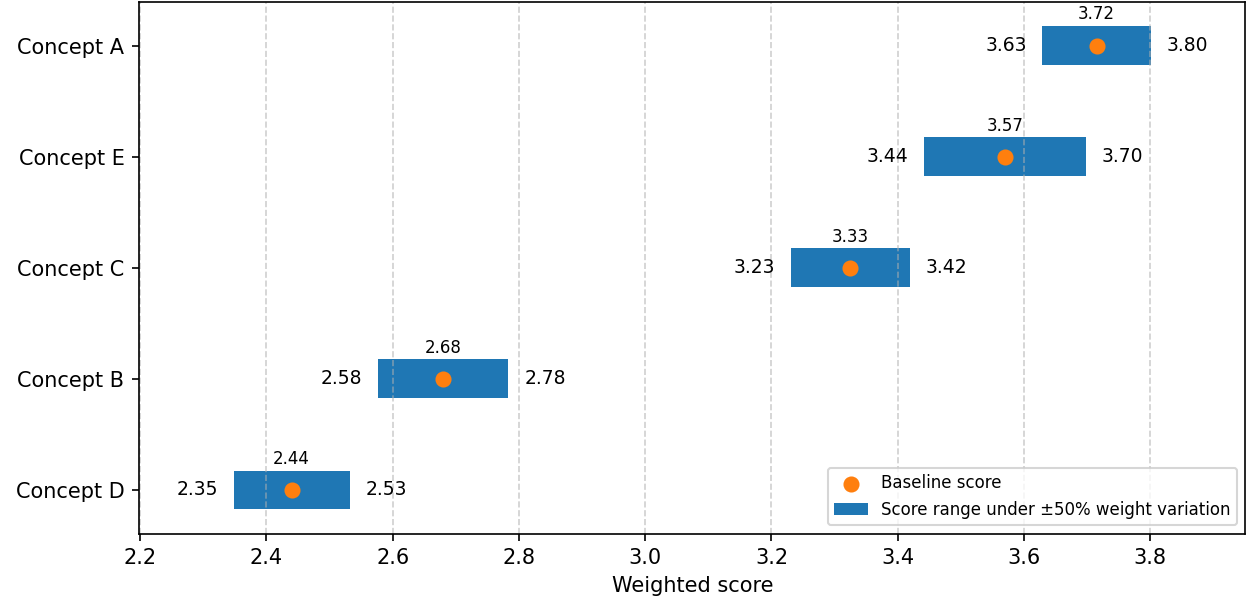
\includegraphics[width=0.6\textwidth]{figures/5050.png}
    \caption{Weighted-score ranges obtained from the relative \(\pm 50\%\) criterion-weight sensitivity analysis.}
    \label{fig:sensitivity_range_plot}
\end{figure}


The figure shows that Concept A remains the highest-scoring concept across the full sensitivity range, with its score varying between approximately 3.63 and 3.80. Concept E remains the closest alternative, with a score range of approximately 3.44 to 3.70. Although the ranking does not change under the tested weight variations, the score ranges of Concept A and Concept E remain close. This confirms that the result is stable in terms of ranking, but not strongly separated numerically.

Concept C remains clearly below the two leading concepts, while Concepts B and D remain lower-ranked across the full sensitivity range. Therefore, the sensitivity analysis supports the selection of Concept A, but also shows that Concept E should be retained as the main backup concept in case later detailed analysis reduces the reliability, performance, or cost confidence of Concept A.



% As shown in \autoref{tab:sensitivity_analysis_weightvariation}, despite these heavy fluctuations, the top ranking remains perfectly unchanged, with Concept A securing 1st place across every single variation.

% \begin{table}[H]
% \centering
% \scriptsize
% \caption{Sensitivity Analysis: Concept Rankings for Relative \(\pm 50\%\) Weight Variation.}
% \label{tab:sensitivity_analysis_weightvariation}
% \setlength{\tabcolsep}{0.001\textwidth}
% \renewcommand{\arraystretch}{1.05}
% \newlength{\sensheaderheight}
% \setlength{\sensheaderheight}{0.040\textwidth}
% \begin{tabularx}{\textwidth}{|
%     >{\hsize=1.500\hsize\raggedright\arraybackslash}X|
%     >{\hsize=0.700\hsize\centering\arraybackslash}X|
%     >{\hsize=0.700\hsize\centering\arraybackslash}X|
%     >{\hsize=0.700\hsize\centering\arraybackslash}X|
%     >{\hsize=0.700\hsize\centering\arraybackslash}X|
%     >{\hsize=0.700\hsize\centering\arraybackslash}X|
% }
% \hline
% \diagbox[
%     width=\dimexpr\hsize+2\tabcolsep+2\arrayrulewidth\relax,
%     height=\sensheaderheight,
%     innerleftsep=0.002\textwidth,
%     innerrightsep=0.002\textwidth
% ]{\textbf{Case}}{\shortstack[r]{\textbf{Rank}}}
% & \makecell{\textbf{Concept}\\\textbf{A}}
% & \makecell{\textbf{Concept}\\\textbf{B}}
% & \makecell{\textbf{Concept}\\\textbf{C}}
% & \makecell{\textbf{Concept}\\\textbf{D}}
% & \makecell{\textbf{Concept}\\\textbf{E}}
% \\ \hline
% \textbf{Baseline Matrix}         & 3.72 (\textbf{1}) & 2.68 (\textbf{4}) & 3.33 (\textbf{3}) & 2.44 (\textbf{5}) & 3.57 (\textbf{2}) \\ \hline
% \textbf{Safety \(+50\%\)}        & 3.78 (\textbf{1}) & 2.62 (\textbf{4}) & 3.27 (\textbf{3}) & 2.42 (\textbf{5}) & 3.66 (\textbf{2}) \\ \hline
% \textbf{Safety \(-50\%\)}        & 3.65 (\textbf{1}) & 2.74 (\textbf{4}) & 3.38 (\textbf{3}) & 2.46 (\textbf{5}) & 3.48 (\textbf{2}) \\ \hline
% \textbf{Reliability \(+50\%\)}   & 3.63 (\textbf{1}) & 2.70 (\textbf{4}) & 3.27 (\textbf{3}) & 2.50 (\textbf{5}) & 3.44 (\textbf{2}) \\ \hline
% \textbf{Reliability \(-50\%\)}   & 3.80 (\textbf{1}) & 2.66 (\textbf{4}) & 3.38 (\textbf{3}) & 2.38 (\textbf{5}) & 3.70 (\textbf{2}) \\ \hline
% \textbf{Cost \(+50\%\)}           & 3.76 (\textbf{1}) & 2.62 (\textbf{4}) & 3.42 (\textbf{3}) & 2.35 (\textbf{5}) & 3.66 (\textbf{2}) \\ \hline
% \textbf{Cost \(-50\%\)}           & 3.67 (\textbf{1}) & 2.74 (\textbf{4}) & 3.23 (\textbf{3}) & 2.53 (\textbf{5}) & 3.48 (\textbf{2}) \\ \hline
% \textbf{Performance \(+50\%\)}    & 3.73 (\textbf{1}) & 2.78 (\textbf{4}) & 3.35 (\textbf{3}) & 2.45 (\textbf{5}) & 3.56 (\textbf{2}) \\ \hline
% \textbf{Performance \(-50\%\)}    & 3.70 (\textbf{1}) & 2.58 (\textbf{4}) & 3.30 (\textbf{3}) & 2.43 (\textbf{5}) & 3.58 (\textbf{2}) \\ \hline
% \textbf{Sustainability \(+50\%\)} & 3.68 (\textbf{1}) & 2.69 (\textbf{4}) & 3.30 (\textbf{3}) & 2.49 (\textbf{5}) & 3.53 (\textbf{2}) \\ \hline
% \textbf{Sustainability \(-50\%\)} & 3.75 (\textbf{1}) & 2.67 (\textbf{4}) & 3.35 (\textbf{3}) & 2.39 (\textbf{5}) & 3.61 (\textbf{2}) \\ \hline
% \end{tabularx}
% \end{table}

In the second check, the weight of each individual criterion is set to zero to determine if a single category dominates the model. The results are compiled in \autoref{fig:eatmap_send_omitting}.

\iffalse

\begin{table}[H]
\centering
\scriptsize
\caption{Sensitivity Analysis: Concept Rankings with Omitted Criteria.}
\label{tab:sensitivity_analysis_zeroweight}
\setlength{\tabcolsep}{0.001\textwidth}
\renewcommand{\arraystretch}{1.05}
\newlength{\sensheaderheight}
\setlength{\sensheaderheight}{0.040\textwidth}
\begin{tabularx}{\textwidth}{|
    >{\hsize=1.500\hsize\raggedright\arraybackslash}X|
    >{\hsize=0.700\hsize\centering\arraybackslash}X|
    >{\hsize=0.700\hsize\centering\arraybackslash}X|
    >{\hsize=0.700\hsize\centering\arraybackslash}X|
    >{\hsize=0.700\hsize\centering\arraybackslash}X|
    >{\hsize=0.700\hsize\centering\arraybackslash}X|
}
\hline
\diagbox[
    width=\dimexpr\hsize+2\tabcolsep+2\arrayrulewidth\relax,
    height=\sensheaderheight,
    innerleftsep=0.002\textwidth,
    innerrightsep=0.002\textwidth
]{\textbf{Omitted}}{\shortstack[r]{\textbf{Rank}}}
& \makecell{\textbf{Concept}\\\textbf{A}}
& \makecell{\textbf{Concept}\\\textbf{B}}
& \makecell{\textbf{Concept}\\\textbf{C}}
& \makecell{\textbf{Concept}\\\textbf{D}}
& \makecell{\textbf{Concept}\\\textbf{E}}
\\ \hline
\textbf{Baseline Matrix} & 3.72 (\textbf{1}) & 2.69 (\textbf{4}) & 3.33 (\textbf{3}) & 2.45 (\textbf{5}) & 3.57 (\textbf{2}) \\ \hline
\textbf{w/o Safety}      & 3.59 (\textbf{1}) & 2.82 (\textbf{4}) & 3.44 (\textbf{2}) & 2.5 (\textbf{5}) & 3.39 (\textbf{3}) \\ \hline
\textbf{w/o Reliability} & 3.88 (\textbf{1}) & 2.64 (\textbf{4}) & 3.44 (\textbf{3}) & 2.32 (\textbf{5}) & 3.83 (\textbf{2}) \\ \hline
\textbf{w/o Cost}        & 3.63 (\textbf{1}) & 2.81 (\textbf{4}) & 3.14 (\textbf{3}) & 2.63 (\textbf{5}) & 3.39 (\textbf{2}) \\ \hline
\textbf{w/o Performance} & 3.69 (\textbf{1}) & 2.49 (\textbf{4}) & 3.27 (\textbf{3}) & 2.43 (\textbf{5}) & 3.59 (\textbf{2}) \\ \hline
\textbf{w/o Sustainability} & 3.79 (\textbf{1}) & 2.68 (\textbf{4}) & 3.37 (\textbf{3}) & 2.35 (\textbf{5}) & 3.65 (\textbf{2}) \\ \hline
\end{tabularx}
\end{table}

\fi


\begin{figure}[H]
    \centering
    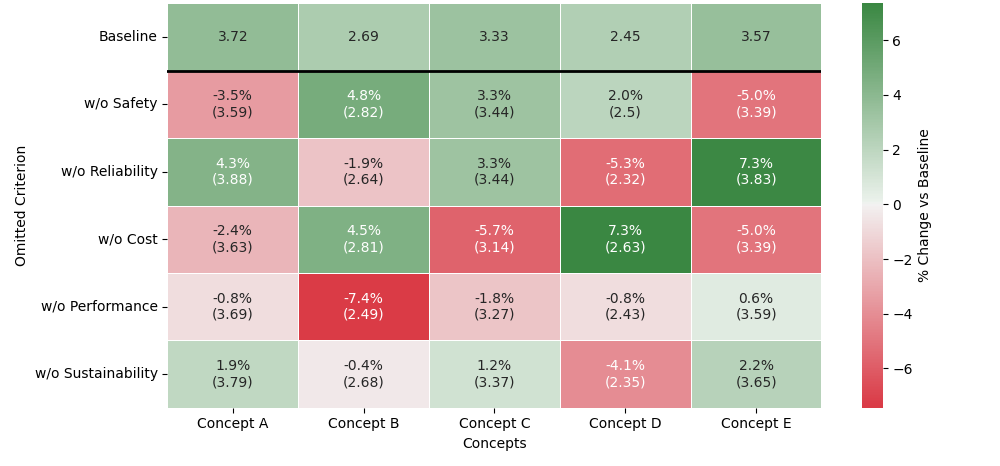
\includegraphics[width=0.8\linewidth]{figures/Heatmap_send_omitting.png}
    \caption{Weighted-score ranges obtained from omitting criteria. Colours according to percentual score change.}
    \label{fig:eatmap_send_omitting}
\end{figure}



 Crucially, when the Cost category is omitted, the artificial compression between the top options disappears as shown in \autoref{tab:rank_percentage_differences_simple_wocost}: Concept A establishes a more robust 7.08\% relative difference over Concept E. Because the cost projection at this stage of development are volatile and subject to high uncertainty, relying on a concept whose competitiveness hinges entirely on cost scores is a major risk. By contrast, Concept A holds a decisive performance premium when financial weights are set aside. Additionally, for all neglected criteria, Concept A ranks first, solidifying its place.

 

\begin{table}[H]
\centering
\scriptsize
\caption{Relative score percentage differences between sequential concept rankings when Cost is omitted.}
\label{tab:rank_percentage_differences_simple_wocost}
\setlength{\tabcolsep}{0.001\textwidth}
\renewcommand{\arraystretch}{1.05}
\setlength{\diffheaderheight}{0.040\textwidth}
\begin{tabularx}{\textwidth}{|
    >{\hsize=1.600\hsize\raggedright\arraybackslash}X|
    >{\hsize=0.850\hsize\centering\arraybackslash}X|
    >{\hsize=0.850\hsize\centering\arraybackslash}X|
    >{\hsize=0.850\hsize\centering\arraybackslash}X|
    >{\hsize=0.850\hsize\centering\arraybackslash}X|
}
\hline
\diagbox[
    width=\dimexpr\hsize+2\tabcolsep+2\arrayrulewidth\relax,
    height=\diffheaderheight,
    innerleftsep=0.002\textwidth,
    innerrightsep=0.002\textwidth
]{\textbf{Comparison}}{\shortstack[r]{\textbf{Value}}}
& \makecell{\textbf{1st to 2nd}\\\textbf{(A $\rightarrow$ E)}}
& \makecell{\textbf{2nd to 3rd}\\\textbf{(E $\rightarrow$ C)}}
& \makecell{\textbf{3rd to 4th}\\\textbf{(C $\rightarrow$ B)}}
& \makecell{\textbf{4th to 5th}\\\textbf{(B $\rightarrow$ D)}}
\\ \hline
\textbf{Percentage Difference} & 7.08\% & 7.96\% & 11.74\% & 6.84\% \\ \hline
\end{tabularx}
\end{table}







\section{Discussion}
The trade-off and subsequent sensitivity analysis demonstrate that Concept A is a robust choice. Although Concept A leads the runner-up, Concept E, by only a narrow baseline margin of 4.20\%, Concept E remains a strong contender. The sensitivity analysis reveals that this proximity stems from cost weighting rather than technical equivalence.


\todo{check if you actually want to add this, its kinda nice}
This interpretation is also supported by a non-parametric statistical comparison of the concept rankings. A Friedman test across the evaluation criteria produced a near-significant result (p=0.054), indicating limited overall separation between the concepts. However, a pairwise Wilcoxon signed-rank test between Concepts A and E showed no statistically significant difference (p=0.465). This suggests that the narrow baseline gap between the two concepts is not caused by consistently superior technical performance of Concept E, but instead by the weighting structure, particularly the strong influence of the Cost criterion.





Concept E's competitiveness relies mostly on its high Cost score (4.6), which compensates for its lower performance in critical engineering categories. Because financial projections at this early stage of development carry high volatility, selecting a design based primarily on cost introduces significant project risk. 

When the Cost category is omitted (\autoref{tab:rank_percentage_differences_simple_wocost}), the margin increases and Concept A establishes a robust 7.08\% score lead over Concept E and consistently ranks first across all isolated engineering criteria. This confirms that Concept A excels in fundamental performance.


Conversely, Concepts B and D can be definitively eliminated; their low rankings are structurally locked across all $\pm 50\%$ weight variations due to severe deficiencies in cost and complexity. While Concept E will be retained as a backup candidate, Concept A provides the most stable, high-performance, and risk-averse foundation for the subsequent Preliminary design phases.
